% !TEX TS-program = pdflatex
% !TeX program = pdflatex
% !TEX encoding = UTF-8
% !TeX spellcheck = en_US

\documentclass[11pt, a4paper]{article}
%\usepackage{fullpage}
\usepackage[left=1cm,right=1cm,top=1cm,bottom=2cm]{geometry}
\usepackage[fleqn]{amsmath}
\usepackage{amssymb}
%\usepackage{indentfirst}
\usepackage[T1]{fontenc}
\usepackage[utf8]{inputenc}
\usepackage[french,english]{babel}
\usepackage{txfonts} 
\usepackage[]{graphicx}
\usepackage{multirow}
\usepackage{hyperref}
\usepackage{parskip}
\usepackage{multicol}
\usepackage{wrapfig}
\usepackage{amssymb}
\usepackage{longtable}
\usepackage{wasysym}


\usepackage{turnstile}%Induction symbole

\usepackage{tikz}
\usetikzlibrary{arrows, automata}
\usetikzlibrary{decorations.pathmorphing}

\renewcommand{\baselinestretch}{1}

\setlength{\parindent}{24pt}


\begin{document}

%\selectlanguage {french}
%\pagestyle{empty} 

\noindent
\begin{tabular}{ll}
\multirow{3}{*}{
\includegraphics[width=1.5cm]{../extra/logo/esi.nlp.pdf}} & 
\'Ecole national Supérieure d'Informatique\\
& 2\textsuperscript{nd} year second cycle (2CSSID)\\
& NLP: Natural Language Processing (2022-2023)
\end{tabular}\\[.25cm]
\noindent\rule{\textwidth}{2pt}\\[-0.5cm]
\begin{center}
{\LARGE \textbf{Tutorial 02: Words semantics}}
\begin{flushright}
	Abdelkrime Aries
\end{flushright}
\end{center}\vspace{-0.5cm}
\noindent\rule{\textwidth}{2pt}

\section*{1. General knowledge}

Given two words W1 and W2, we want to determine their relation's type based on their different representations.
Let us note:
\begin{itemize}
	\item \textbf{HYP(W1, W2)}: a measure based on the shorter path connecting W1 and W2 using hyponym/hyperonym Wordnet relations.
	\item \textbf{COS(X, Y)}: Cosine similarity between two vectors X and Y.
	\item \textbf{OneHot(W)}: OneHot representation of a word W.
	\item \textbf{TermTerm(W)}: erm-Term representation of a word W.
\end{itemize}

\noindent
Select the captured relation's type for each measure (justify):
\begin{center}
	\begin{tabular}{|llll|}
	\hline 
	Measure & Semantic similarity & Association & None\\
	\hline
	HYP(W1, W2) & \Square & \Square & \Square \\
	COS(OneHot(W1), OneHot(W2)) & \Square & \Square & \Square \\
	COS(TermTerm(W1), TermTerm(W2)) & \Square & \Square & \Square \\
	\hline
	\end{tabular}
\end{center}

\section*{2. Lexical databases}

Here is an excerpt from WordNet:

\noindent
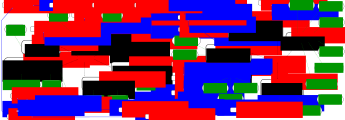
\includegraphics[width=\textwidth]{../img/word-sem/wn-exp.pdf}

\noindent
Given these sentences containing the words "fish" and "chicken":

\begin{center}
	\begin{tabular}{|ll|}
	\hline 
	(1) I had chicken for dinner & (2) River's fish are not delicious \\
	(3) Fish is a zodiac sign & (4) Astrologically speaking, I am not a fish \\
	(5) Sea contains all kind of fish & (6) We have chicken at home \\
	(7) That kid is a chicken & (8) I fish on the river\\
	\hline
\end{tabular}
\end{center}

\begin{enumerate}
	\item Substitute the two words in each sentence, keeping the meaning.
	
	\item Calculate Path-similarity between the following words tuples: (1.chicken, 2.fish) ; (3.fish, 4.fish) ; (5.fish, 6.chicken) ; (7.chicken, 8.fish) ; (6.chicken, 7.chicken) ; (1.chicken, 5.fish) ; (2.fish, 6.chicken). If no relation is present, the similarity is 0.
	\item For these tuples, mention the nearest common ancestor.
	\item Try to replace the sentences' words by this ancestor. What do you notice ?
\end{enumerate}


\section*{3. Vector representation of words}

We have these 3 sentences: 

\begin{center}
	\begin{tabular}{|lll|}
	\hline 
	I fish a fish in the river & the river where I fish is far & fish live in the river\\
	\hline
\end{tabular}
\end{center}

\begin{enumerate}
	\item Using TF representation, 
	\begin{itemize}
		\item encode these sentences (words ordered alphabetically);
		\item calculate cosine similarity between each two of them;
		\item and calculate cosine similarity between the words: "far", "fish", "live" and "river".
	\end{itemize}

	\item Apply stop-words filtering and redo the same thing. Stop-words are [ I, a, in, the, is, where ].
	
	\item Using Term-term representation, 
	\begin{itemize}
		\item encode all words using a co-occurrence window of 2-2 (words ordered alphabetically);
		\item find each sentence's encoding using the centroid of its words;
		\item calculate cosine similarity between each two of the sentences;
		\item and calculate cosine similarity between the words: "far", "fish", "live" and "river".
	\end{itemize}

	\item Using correlation measure (Pearson, Spearman or Kendall), 
	\begin{itemize}
		\item calculate correlation between words cosine similarities based on TF with those based on Term-term;
		\item calculate correlation between sentences cosine similarities based on TF with those based on Term-term;
		\item what can we conclude?
	\end{itemize}
	
\end{enumerate}

\section*{4. Word embedding}

\textbf{\textit{In this part, you can either calculate manually or implement the models using a programming language.}}

\noindent Using these sentences:
\begin{center}
	\begin{tabular}{|lll|}
		\hline 
		I fish a fish in the river & the river where I fish is far & fish live in the river\\
		\hline
	\end{tabular}
\end{center}

\begin{enumerate}
	\item Use the token \textbf{\textless s \textgreater} to indicate a sentence's start and ending.
	\item Train a Word2Vec (CBOW) model which estimates a word given two words (pre-, post-):
	\begin{itemize}
		\item each word is encoded as a 2 values vector;
		\item all weights are initialized to 1;
		\item simple normalization is used as activation function instead of softmax;
		\item cross-entropy without log function is used as cost function (I know ... it is not cross entropy anymore);
		\item 1 iteration.
	\end{itemize}
	
	\item Train a Word2Vec (Skip-gram) model which estimates two words (pre-, post-) given a word using the same parameters.
	
	\item What is the encoding of the words: "fish" and "river" using these two models?
	\item Calculate cosine similarity between these two words using these two models. 
	
	\item Train a BERT-like model using these parameters (either code it or manually calculate):
	\begin{itemize}
		\item each word is encoded using three vectors: vocabulary (different words plus other tokens), position (10 max) and part (2);
		\item Tokens are encoded alphabetically (special tokens start with \textbf{[});
		\item each of these vectors is embedded into a two-values vector;
		\item hidden layers have no activation function (or rather, it is the identity one);
		\item just one head attention with a layer of two neurons at the end;
		\item simple normalization is used as activation function instead of softmax;
		\item all weights are initialized to 1;
		\item cross-entropy without log function is used as cost function (I know ... it is not cross entropy anymore);
		\item task1: Sentence completion; for each 3 words, detect if the rest from all sentences is its completion (S1-S1, S1-S2, S1-S3, S2-S1, S2-S2, S2-S3, S3-S1, S3-S1, S3-S3); 
		\item task2: Masked language model; For the first sample, we mask the first word, the second sample, the second word and so on;
		\item 1 iteration.
	\end{itemize}
	
\end{enumerate}





\end{document}
